\section{ПРОГРАМНА РЕАЛІЗАЦІЯ СИСТЕМИ ДЛЯ УПРАВЛІННЯ КОРИСТУВАЧАМИ, ДОКУМЕНТАМИ, ЗАВДАННЯМИ І МОЖЛИВОСТІ СПІЛЬНОЇ РОБОТИ}
\subsection{Реалізація роботи бази даних}
\par Загальна структура бази даних зображено на рисунку \ref{pic:db_shema}. Весь код для створення бази даних реалізовано мовою SQL, за допомогою запитів до БД.
\par Зовнішні посилання створено за допомогою команди Reference. Для прикладу код для створення таблиці користувачів (worker), котра має чотири зовнішні ключі які посилаються на таблиці команди (team), роль користувача (role\_name), тип посади (job\_type\_name) та регіон (region\_name).

\par Відповідно таким чином і реалізовано всі решта таблиць. Код для створення таблиці таблиці користувачів:
\begin{lstlisting}[language=SQL]
DROP TABLE IF EXISTS `worker`;
/*!40101 SET @saved_cs_client     = @@character_set_client */;
/*!40101 SET character_set_client = utf8 */;
CREATE TABLE `worker` (
  `id` bigint(20) NOT NULL AUTO_INCREMENT,
  `birthday` date DEFAULT NULL,
  `date_hire` date DEFAULT NULL,
  `login` varchar(255) NOT NULL,
  `name` varchar(255) NOT NULL,
  `pass` varchar(255) NOT NULL,
  `phone` varchar(255) DEFAULT NULL,
  `photo` longblob,
  `private_mail` varchar(255) DEFAULT NULL,
  `street` varchar(255) DEFAULT NULL,
  `surname` varchar(255) NOT NULL,
  `version` int(11) DEFAULT NULL,
  `job_type_name` bigint(20) NOT NULL,
  `region_name` bigint(20) NOT NULL,
  `role_name` bigint(20) DEFAULT NULL,
  `team_name` bigint(20) NOT NULL,
  `mobile` varchar(255) DEFAULT NULL,
  PRIMARY KEY (`id`),
  UNIQUE KEY `login` (`login`),
  KEY `FKD162537E30271785` (`team_name`),
  KEY `FKD162537EB0DD720C` (`job_type_name`),
  KEY `FKD162537E520C2F83` (`role_name`),
  KEY `FKD162537EBDECCB25` (`region_name`),
  CONSTRAINT `FKD162537E30271785` FOREIGN KEY (`team_name`) REFERENCES `team` (`id`),
  CONSTRAINT `FKD162537E520C2F83` FOREIGN KEY (`role_name`) REFERENCES `worker_role` (`id`),
  CONSTRAINT `FKD162537EB0DD720C` FOREIGN KEY (`job_type_name`) REFERENCES `worker_job_type` (`id`),
  CONSTRAINT `FKD162537EBDECCB25` FOREIGN KEY (`region_name`) REFERENCES `region` (`id`)
) ENGINE=InnoDB AUTO_INCREMENT=3 DEFAULT CHARSET=utf8;
/*!40101 SET character_set_client = @saved_cs_client */;	
\end{lstlisting}
\par Посилання на інші таблиці на веб інтерфейсі реалізовано за допомогою випадаючих списків -- це дає можливість забезпечити введення вірних даних і допомагає відобразити вже існуючі в базі даних записи.
Для прикладу візьмемо форму для створення нового користувача та вибору регіону, що зображено на рисунку \ref{pic:page_drop_down}.


\begin{figure}[!ht]
\centering
    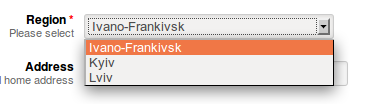
\includegraphics[width=0.5\textwidth]{page_drop_down.png}
    \captionof{figure}{Вибір регіону при створенні користувача}\label{pic:page_drop_down}
\end{figure}


\subsection{Реалізація веб інтерфейсу}
\par Веб інтерфейс користувача повинний бути зручний та інтуїтивно зрозумілий кожному користувачеві, тому його було реалізовано в легких тонах та зручно розташовано всі навігаційні елементи.

\begin{figure}[!ht]
\centering
		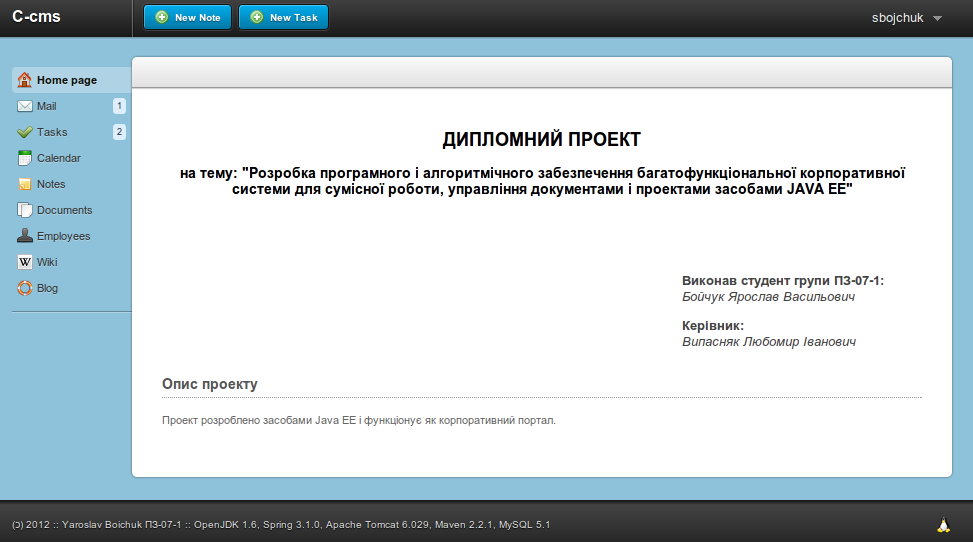
\includegraphics[width=1.00\textwidth]{page_main.png}
		\captionof{figure}{Загальний інтерфейс програмного продукту}\label{pic:page_main}
\end{figure}


\subsubsection{Навігаційна панель}
\par На навігаційній панелі розташовані елементи швидкого доступу до завдань та задач.

\subsubsection{Головне меню}
\par Навігація по веб ресурсу реалізована за допомогою головного меню. В головному меню відображаються всі доступні на сайті навігаційні посилання:
\begin{enumerate}
  \item головна сторінка;
  \item корпоративна пошта;
  \item завдання;
  \item календар;
  \item нотатки;
  \item документи;
  \item список робочих;
  \item корпоративна вікі;
  \item блог.
\end{enumerate}
\par При переході на будь-яке меню, воно зразу підсвічується -- це зроблено для зручності користувачеві, щоб було зразу видно де він знаходиться в даний момент часу. Програмно це відбувається за допомогою передачі з контролера в модель атрибута із назвою меню:
\begin{lstlisting}[language=Java]
uiModel.addAttribute("menu", "NOTE");
\end{lstlisting}
Потім в JSP вигляді головного меню відбувається перевірка на значення поточного меню, і якщо воно сходиться із атрибутом <<menu>> то додається css клас <<active>>:
\lstinputlisting[language=XML]{code/menu_active.jspx}

\begin{figure}[!ht]
\centering
    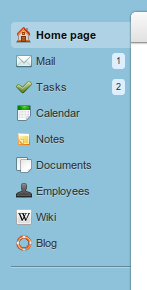
\includegraphics[width=1.00\textwidth]{page_menu.png}
    \captionof{figure}{Навігаційне меню порталу}\label{pic:page_menu}
\end{figure}








